\chapter{Thermo-optical topology optimization problems}\label{chap:to}
%CHECK COPYRIGHT FOR FIGURES AND REPRINTS
%In this chapter we will focus on the effects of multiphysics couplings in nanophotonic devices, reviewing state-of-the-art research, 
%highlighting open topology optimization problems, and presenting our contributions to the field.
%We will focus on three main classes of multiphysics couplings: thermo-optical, opto-mechanical, and electro-optical systems.
%\begin{figure}[tb]
%    \centering
%    \makebox[\textwidth][c]{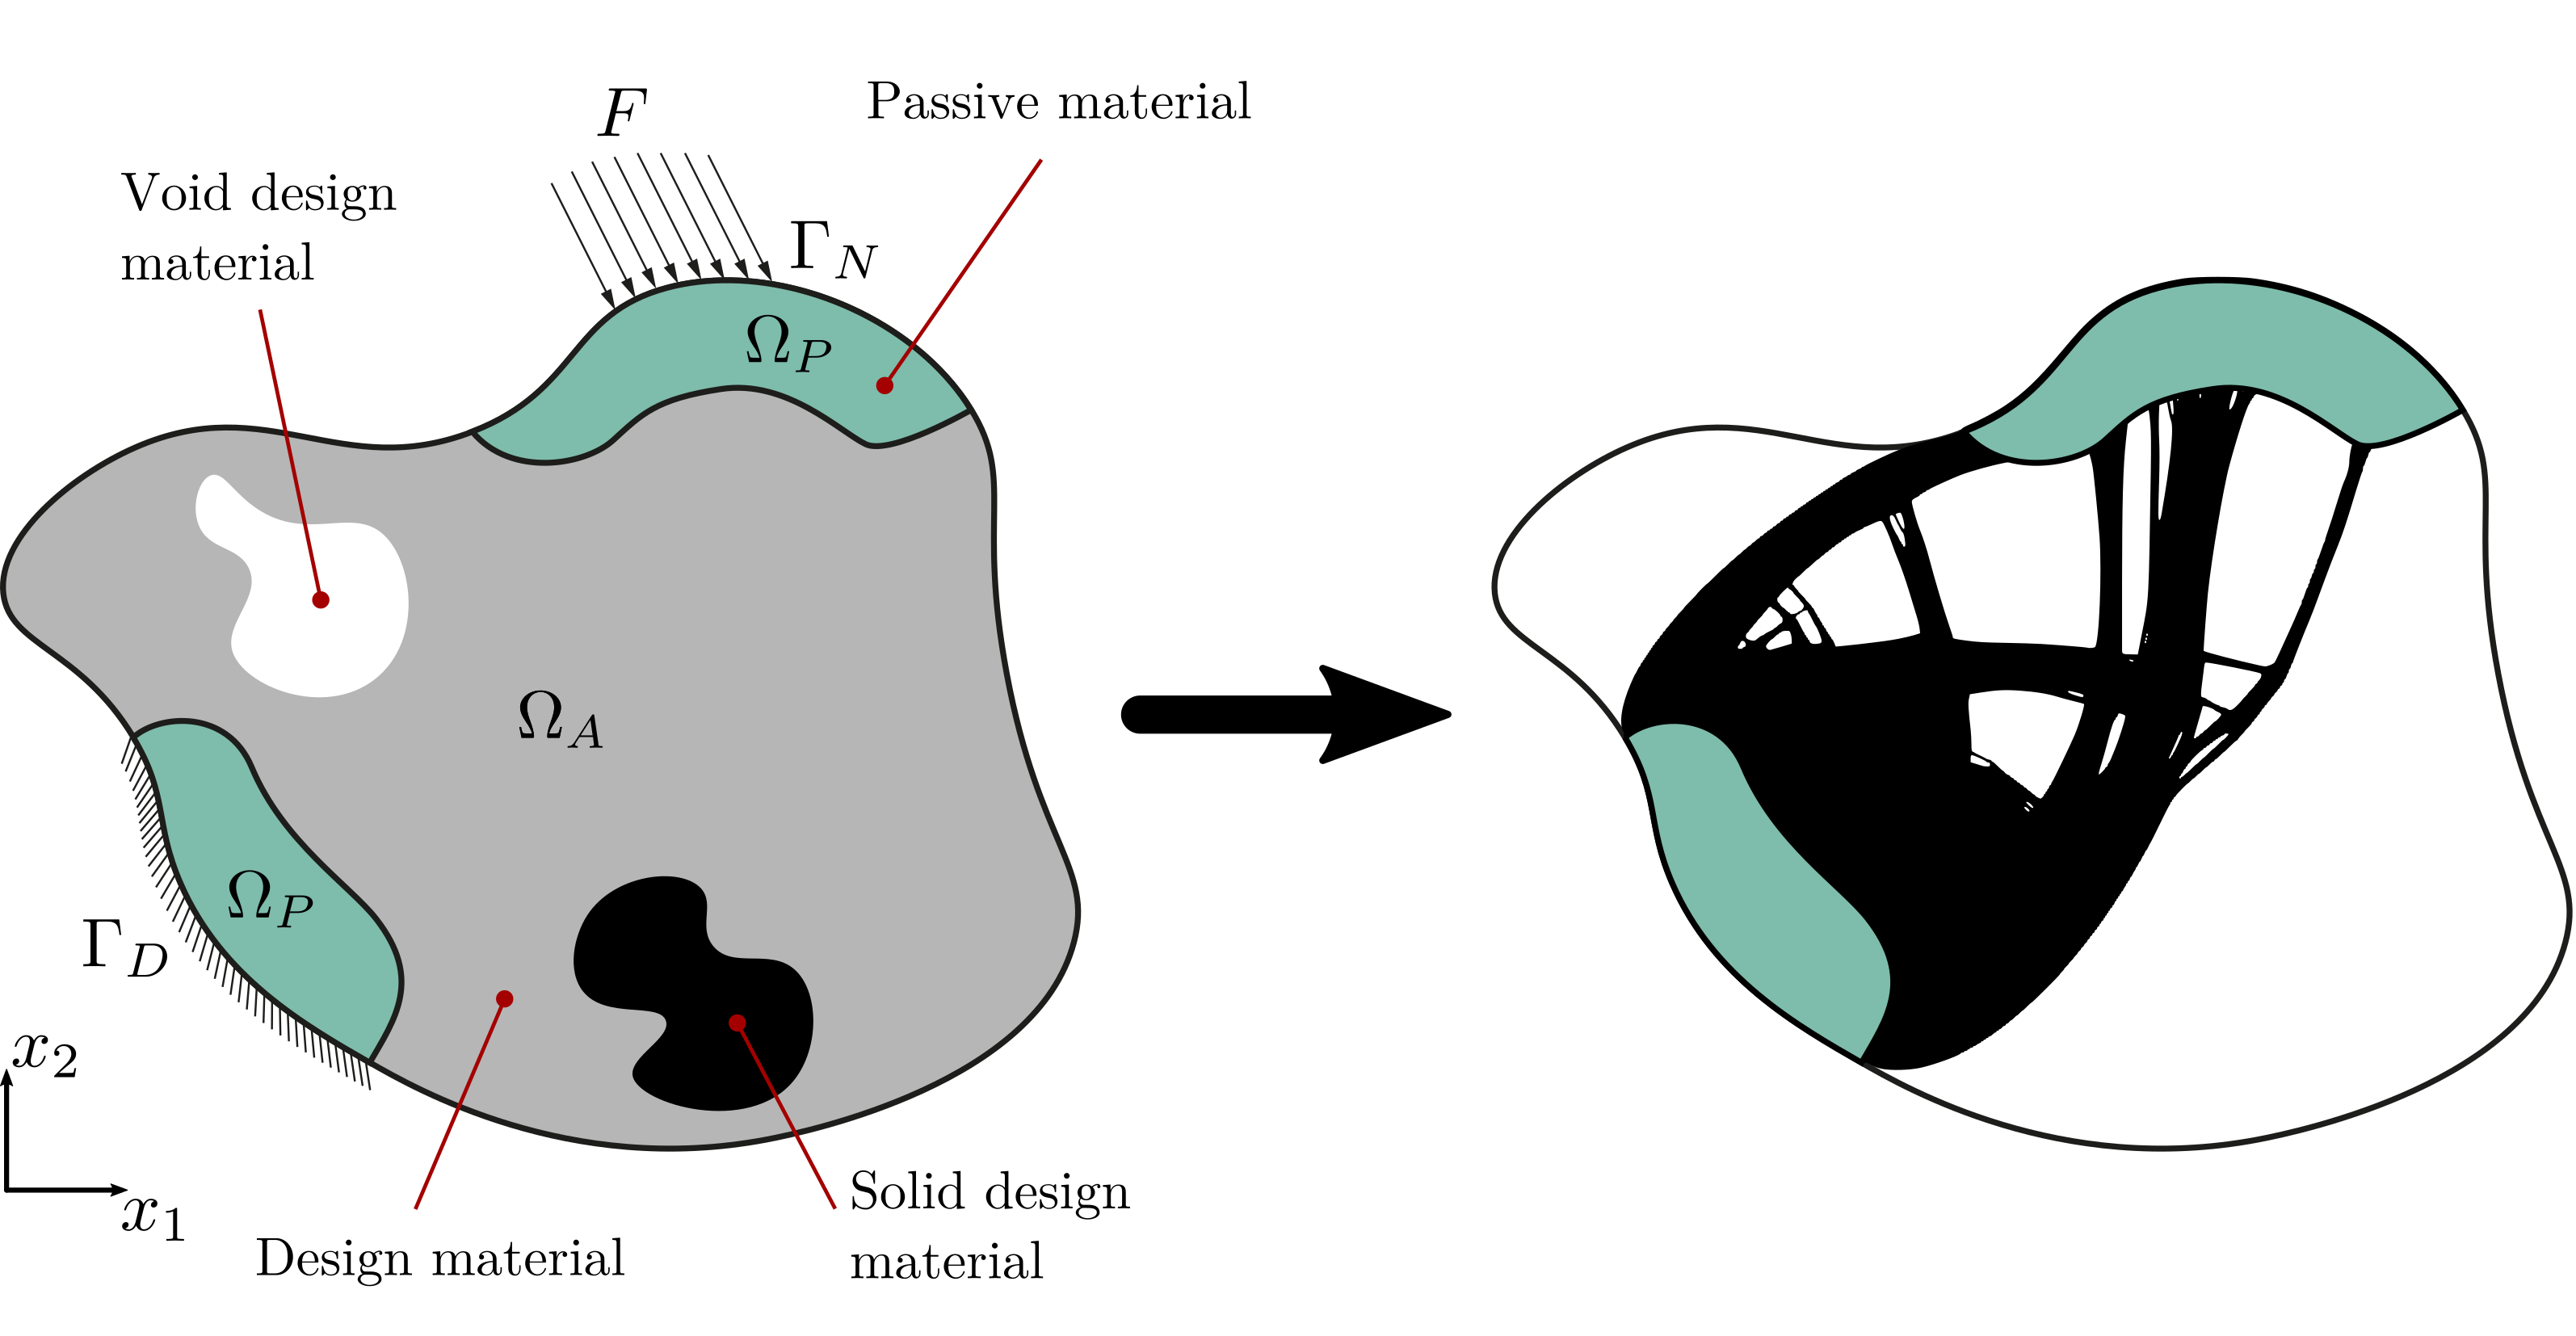
\includegraphics[width=1\imwidth]{figures/simpModel.png}}%
%    \caption{Bla bla bla...}
%    \label{fig:illustateTopOpt}
%\end{figure
%\begin{equation}
%    (EIu'')'' = q
%\end{equation}
%\beginfigure}[tb]
%    \centering
%    \makebox[\textwidth][c]{\begin{tikzpicture}[remember picture]
    \begin{scope}[xshift=0mm]
        % angle (deg)
        \newcommand\ai{10}
        % line width
        \newcommand\wi{1pt}
        % cell size
        \newcommand\cellsize{3}
        % Rank-$N$ size
        \newcommand\di{0.75}

        % cell
        \draw[gray!10,   fill=gray!10, rotate around={\ai:(0,0)}] (0,0) rectangle (\cellsize,\cellsize) node (rect1) {};
        \draw[black!60, fill=black!60, rotate around={\ai:(0,0)}] (0,0) rectangle (\di,\cellsize);

        % orientation frame
        \draw[black, -stealth, line width=\wi, rotate around={\ai:({\di*cos(\ai) - \cellsize/2*sin(\ai)},{\di*sin(\ai) + \cellsize/2*cos(\ai)})}] ({\di*cos(\ai) - \cellsize/2*sin(\ai)},{\di*sin(\ai) + \cellsize/2*cos(\ai)}) -- ({\di*cos(\ai) - \cellsize/2*sin(\ai) + 0.75},{\di*sin(\ai) + \cellsize/2*cos(\ai)});
        \draw[black, -stealth, line width=\wi, rotate around={\ai:({\di*cos(\ai) - \cellsize/2*sin(\ai)},{\di*sin(\ai) + \cellsize/2*cos(\ai)})}] ({\di*cos(\ai) - \cellsize/2*sin(\ai)},{\di*sin(\ai) + \cellsize/2*cos(\ai)}) -- ({\di*cos(\ai) - \cellsize/2*sin(\ai)},{\di*sin(\ai) + \cellsize/2*cos(\ai) + 0.75});

        % local frame
        \draw[black, -stealth, dashed, line width=\wi] (0,0) -- ({\cellsize + 0.8},0);
        \draw[black, -stealth, dashed, line width=\wi] (0,0) -- (0,{\cellsize + 0.8});

        % ruler
        \draw[black, |-|, line width=\wi, rotate around={\ai:(0,0)}] (0,0) -- (\cellsize,0);
        \draw[black,  -|, line width=\wi, rotate around={\ai:(0,0)}] (0,0) -- (\di,0);

        % arc
        \draw[black, dotted, line width=\wi] (\cellsize,0) arc (0:\ai:\cellsize);

        % annotation
        \draw (\cellsize + 0.7, -0.3) node {$x_1 / \epsilon^3$};
        \draw (-0.5, \cellsize + 0.8) node {$x_2 / \epsilon^3$};
        \draw (\cellsize/2,-0.75) node {Rank-$1$};

        \draw[rotate around={{\ai/2}:(0,0)}] ({\cellsize+0.3},0) node {$\theta_1$};

        \draw[rotate around={{\ai}:(0,0)}] ({\di/2},0.4) node [rotate around={{\ai}:(0,0)}] {$\mu_1$};
        \draw[rotate around={{\ai}:(0,0)}] ({(\cellsize - \di)/2 + \di},0.4) node [rotate around={{\ai}:(0,0)}] {$1-\mu_1$};

        \draw[rotate around={{\ai}:(0,0)}] ({0+0.4},{\cellsize-0.4}) node [rotate around={{\ai}:(0,0)}] {$(+)$};
        \draw[rotate around={{\ai}:(0,0)}] ({\cellsize-0.4},{\cellsize-0.4}) node [rotate around={{\ai}:(0,0)}] {$(-)$};
        \coordinate (A) at (rect1.north);


        \draw[rotate around={\ai:({\di*cos(\ai) - \cellsize/2*sin(\ai)},{\di*sin(\ai) + \cellsize/2*cos(\ai)})}] ({\di*cos(\ai) - \cellsize/2*sin(\ai)+1} , {\di*sin(\ai) + \cellsize/2*cos(\ai) + 0.2}) node {$\mathbf{n}_1$};
        \draw[rotate around={\ai:({\di*cos(\ai) - \cellsize/2*sin(\ai)},{\di*sin(\ai) + \cellsize/2*cos(\ai)})}] ({\di*cos(\ai) - \cellsize/2*sin(\ai) + 0.3} , {\di*sin(\ai) + \cellsize/2*cos(\ai) + 1}) node {$\mathbf{m}_1$};



    \end{scope}
    \begin{scope}[xshift=45mm]
        % angle (deg)
        \newcommand\ai{15}
        % line width
        \newcommand\wi{1pt}
        % cell size
        \newcommand\cellsize{3}
        % Rank-$N$ size
        \newcommand\di{0.6}

        % cell
        \draw[gray!40,   fill=gray!40, rotate around={\ai:(0,0)}] (0,0) rectangle (\cellsize,\cellsize) node (rect2) {};
        \draw[black!60, fill=black!60, rotate around={\ai:(0,0)}] (0,0) rectangle (\di,\cellsize);

        % orientation frame
        \draw[black, -stealth, line width=\wi, rotate around={\ai:({\di*cos(\ai) - \cellsize/2*sin(\ai)},{\di*sin(\ai) + \cellsize/2*cos(\ai)})}] ({\di*cos(\ai) - \cellsize/2*sin(\ai)},{\di*sin(\ai) + \cellsize/2*cos(\ai)}) -- ({\di*cos(\ai) - \cellsize/2*sin(\ai) + 0.75},{\di*sin(\ai) + \cellsize/2*cos(\ai)});
        \draw[black, -stealth, line width=\wi, rotate around={\ai:({\di*cos(\ai) - \cellsize/2*sin(\ai)},{\di*sin(\ai) + \cellsize/2*cos(\ai)})}] ({\di*cos(\ai) - \cellsize/2*sin(\ai)},{\di*sin(\ai) + \cellsize/2*cos(\ai)}) -- ({\di*cos(\ai) - \cellsize/2*sin(\ai)},{\di*sin(\ai) + \cellsize/2*cos(\ai) + 0.75});

        % local frame
        \draw[black, -stealth, dashed, line width=\wi] (0,0) -- ({\cellsize + 0.8},0);
        \draw[black, -stealth, dashed, line width=\wi] (0,0) -- (0,{\cellsize + 0.8});

        % ruler
        \draw[black, |-|, line width=\wi, rotate around={\ai:(0,0)}] (0,0) -- (\cellsize,0);
        \draw[black,  -|, line width=\wi, rotate around={\ai:(0,0)}] (0,0) -- (\di,0);

        % arc
        \draw[black, dotted, line width=\wi] (\cellsize,0) arc (0:\ai:\cellsize);

        % annotation
        \draw (\cellsize + 0.7, -0.3) node {$x_1 / \epsilon^2$};
        \draw (-0.5, \cellsize + 0.8) node {$x_2 / \epsilon^2$};
        \draw (\cellsize/2,-0.75) node {Rank-$2$};

        \draw[rotate around={{\ai/2}:(0,0)}] ({\cellsize+0.3},0) node {$\theta_2 + \pi/4$};

        \draw[rotate around={{\ai}:(0,0)}] ({\di/2},0.4) node [rotate around={{\ai}:(0,0)}] {$\mu_2$};
        \draw[rotate around={{\ai}:(0,0)}] ({(\cellsize - \di)/2 + \di},0.4) node [rotate around={{\ai}:(0,0)}] {$1-\mu_2$};

        \draw[rotate around={{\ai}:(0,0)}] ({0+0.4},{\cellsize-0.4}) node [rotate around={{\ai}:(0,0)}] {$(+)$};
        \draw[rotate around={{\ai}:(0,0)}] ({\cellsize-0.9},{\cellsize-0.4}) node [rotate around={{\ai}:(0,0)}] (B) {$(\text{Rank-1})$};
        \coordinate (B2) at (rect2.north);


        \draw[rotate around={\ai:({\di*cos(\ai) - \cellsize/2*sin(\ai)},{\di*sin(\ai) + \cellsize/2*cos(\ai)})}] ({\di*cos(\ai) - \cellsize/2*sin(\ai)+1} , {\di*sin(\ai) + \cellsize/2*cos(\ai) + 0.2}) node {$\mathbf{n}_2$};
        \draw[rotate around={\ai:({\di*cos(\ai) - \cellsize/2*sin(\ai)},{\di*sin(\ai) + \cellsize/2*cos(\ai)})}] ({\di*cos(\ai) - \cellsize/2*sin(\ai) + 0.3} , {\di*sin(\ai) + \cellsize/2*cos(\ai) + 1}) node {$\mathbf{m}_2$};


    \end{scope}
    \begin{scope}[xshift=90mm]
        % angle (deg)
        \newcommand\ai{20}
        % line width
        \newcommand\wi{1pt}
        % cell size
        \newcommand\cellsize{3}
        % Rank-$N$ size
        \newcommand\di{1.0}

        % cell
        \draw[gray!60,   fill=gray!60, rotate around={\ai:(0,0)}] (0,0) rectangle (\cellsize,\cellsize);
        \draw[black!60, fill=black!60, rotate around={\ai:(0,0)}] (0,0) rectangle (\di,\cellsize);

        % orientation frame
        \draw[black, -stealth, line width=\wi, rotate around={\ai:({\di*cos(\ai) - \cellsize/2*sin(\ai)},{\di*sin(\ai) + \cellsize/2*cos(\ai)})}] ({\di*cos(\ai) - \cellsize/2*sin(\ai)},{\di*sin(\ai) + \cellsize/2*cos(\ai)}) -- ({\di*cos(\ai) - \cellsize/2*sin(\ai) + 0.75},{\di*sin(\ai) + \cellsize/2*cos(\ai)});
        \draw[black, -stealth, line width=\wi, rotate around={\ai:({\di*cos(\ai) - \cellsize/2*sin(\ai)},{\di*sin(\ai) + \cellsize/2*cos(\ai)})}] ({\di*cos(\ai) - \cellsize/2*sin(\ai)},{\di*sin(\ai) + \cellsize/2*cos(\ai)}) -- ({\di*cos(\ai) - \cellsize/2*sin(\ai)},{\di*sin(\ai) + \cellsize/2*cos(\ai) + 0.75});

        % local frame
        \draw[black, -stealth, dashed, line width=\wi] (0,0) -- ({\cellsize + 0.8},0);
        \draw[black, -stealth, dashed, line width=\wi] (0,0) -- (0,{\cellsize + 0.8});

        % ruler
        \draw[black, |-|, line width=\wi, rotate around={\ai:(0,0)}] (0,0) -- (\cellsize,0);
        \draw[black,  -|, line width=\wi, rotate around={\ai:(0,0)}] (0,0) -- (\di,0);

        % arc
        \draw[black, dotted, line width=\wi] (\cellsize,0) arc (0:\ai:\cellsize);

        % annotation
        \draw (\cellsize + 0.7, -0.3) node {$x_1 / \epsilon$};
        \draw (-0.5, \cellsize + 0.8) node {$x_2 / \epsilon$};
        \draw (\cellsize/2,-0.75) node {Rank-$3$};

        \draw[rotate around={{\ai/2}:(0,0)}] ({\cellsize+0.3},0) node {$\theta_3 - \pi/2$};

        \draw[rotate around={{\ai}:(0,0)}] ({\di/2},0.4) node [rotate around={{\ai}:(0,0)}] {$\mu_3$};
        \draw[rotate around={{\ai}:(0,0)}] ({(\cellsize - \di)/2 + \di},0.4) node [rotate around={{\ai}:(0,0)}] {$1-\mu_3$};

        \draw[rotate around={{\ai}:(0,0)}] ({0+0.4},{\cellsize-0.4}) node [rotate around={{\ai}:(0,0)}] {$(+)$};
        \draw[rotate around={{\ai}:(0,0)}] ({\cellsize-0.9},{\cellsize-0.4}) node [rotate around={{\ai}:(0,0)}] (C) {$(\text{Rank-2})$};


        \draw[rotate around={\ai:({\di*cos(\ai) - \cellsize/2*sin(\ai)},{\di*sin(\ai) + \cellsize/2*cos(\ai)})}] ({\di*cos(\ai) - \cellsize/2*sin(\ai)+1} , {\di*sin(\ai) + \cellsize/2*cos(\ai) + 0.2}) node {$\mathbf{n}_3$};
        \draw[rotate around={\ai:({\di*cos(\ai) - \cellsize/2*sin(\ai)},{\di*sin(\ai) + \cellsize/2*cos(\ai)})}] ({\di*cos(\ai) - \cellsize/2*sin(\ai) + 0.3} , {\di*sin(\ai) + \cellsize/2*cos(\ai) + 1}) node {$\mathbf{m}_3$};

    \end{scope}
    \path[-latex,black,thick] (A) edge [bend left=50] (B);
    \path[-latex,black,thick] (B2) edge [bend left=50] (C);
\end{tikzpicture}}%
%    \caption{Bla bla bla...}
%    \label{fig:Rank}
%\end{figure}
%\section{Coupled optical systems}
%TODO: Include if we end up doing the Green's function study.
% Make a connection to the Green's function formalism and derive system of coupled equations.
%\section{Thermo-optical systems~\cite{ownpub0}}\label{sec:thermo_optical}
Thermo-optical systems exploit the interplay between temperature and electromagnetic fields to enable active control over optical properties. 
The primary mechanism behind this coupling is the thermo-optic effect, 
in which the refractive index of a material changes as a function of temperature. 
This effect plays a central role in many integrated photonics applications, such as
 optical phase shifters~\cite{TOPS_1, TOPS_2, TOPS_3}, reconfigurable photonic circuits~\cite{program, PIC}, and thermally tunable switches~\cite{switch, switch_2} and filters~\cite{filter}.

 Despite their broad application, thermo-optical devices are still difficult to optimize due to the intricate interplay between thermal and optical physics.
  Topology optimization offers a systematic design optimization solution, with application examples in
 thermo-optical phase shifters~\cite{TOPS_heat, ownpub0}, optical mirror-like thermo-mechanical structures~\cite{opt_perf}, and
structural integrity constraints~\cite{structural_heat}, among others.

In the following sections, we provide an overview of how to model and optimize thermo-optic systems, 
focusing on our research contribution~\cite{ownpub0}, which extends previous thermo-optic topology 
optimization methods by explicitly incorporating the coupling between heat transfer and optics.

\section{The thermo-optic effect}\label{sec:to_effect}

To model the coupled thermo-optical topology optimization problem, we combine the governing equation of the optical model (\eqref{eq:wave_eq})
with a heat transfer model. The simplest heat transfer model is the steady-state heat equation, which describes the
heat transfer in a medium due to conduction and heat sources. The steady-state \textbf{heat equation} is given by
\begin{equation}\label{eq:heat}
 -\nabla \cdot \left[ G(\mathbf{r})\cdot \nabla T(\mathbf{r}) \right] = Q(\mathbf{r})\,,
\end{equation}
where $T$ is the temperature, $G$ is the thermal conductivity, and $Q$ is a volumetric heat source. This equation can be
extended by considering convection and radiation effects, which may be important in some thermo-optical systems.

Temperature can be coupled to the optical response via the \textbf{thermo-optic coefficient} (TOC), which relates the local temperature field
to changes in the material's refractive index. This is typically approximated by the linear relation\footnote{Large temperature gradients may lead to nonlinear effects, requiring higher order terms.}
\begin{equation}
n(\mathbf{r}) = n_0 + \text{TOC} \cdot \left[T(\mathbf{r}) - T_0\right],
\end{equation}
where $n_0$ and $T_0$ are the reference (unheated) refractive index and reference temperature, respectively. Thus, to solve a problem that is weakly coupled via the TOC, one first solves the heat equation
in \eqref{eq:heat}
to determine the temperature profile, which can be used to determine
the spatially varying refractive index. The temperature-dependent refractive index is then used in \eqref{eq:wave_eq} to find the optical field.

\section{Topology optimization of thermo-optical phase shifters~\cite{ownpub0}}\label{sec:TOPS}

Among the many applications that utilize the thermo-optic coefficient, we find integrated photonic circuit components, which rely on the large 
TOC of silicon ($\text{TOC} \approx 1.8 \cdot 10^{-4}\, \text{K}^{-1}$) at room-temperature ($\approx300$ K) and telecom wavelength 
($\lambda=1.55$ \textmu m)~\cite{thermo-optic-coef}. One of those components is the \textbf{thermo-optical phase shifter}, which, as shown in \figref{fig:thermo_res} (a),
uses a heating device to locally modify the refractive index of a waveguide structure to induce a phase shift ($\Delta \Phi$) in the propagating optical mode
\begin{equation}\label{eq:phase_shift}
\Delta \Phi = \frac{2\pi L}{\lambda} \Delta n_\text{eff}\,,
\end{equation}
where $L$ is the device length and $\Delta n_\text{eff} = n_\text{eff, heated} - n_\text{eff, unheated}$
 is the change of the effective refractive index of the guided mode. 
 
 It is not straightforward to design thermo-optical phase shifters. Ideally, one would like to place a heater close to the waveguide to achieve a phase shift with minimum input power.
 Theoretically, this would imply positioning the metal in contact to the waveguide to ensure efficient heat transfer, but since the heaters are usually metallic ($\kappa > 0$, in \eqref{eq:perm}), this would result
 in optical losses. As shown in the optical and thermal responses in \figref{fig:thermo_res} (b), this trade-off problem can be tackled with topology optimization to design efficient low-loss thermo-optical phase shifters, 
 as we will detail in the following sections.

\begin{figure}[tb]
    \centering
    \makebox[\textwidth][c]{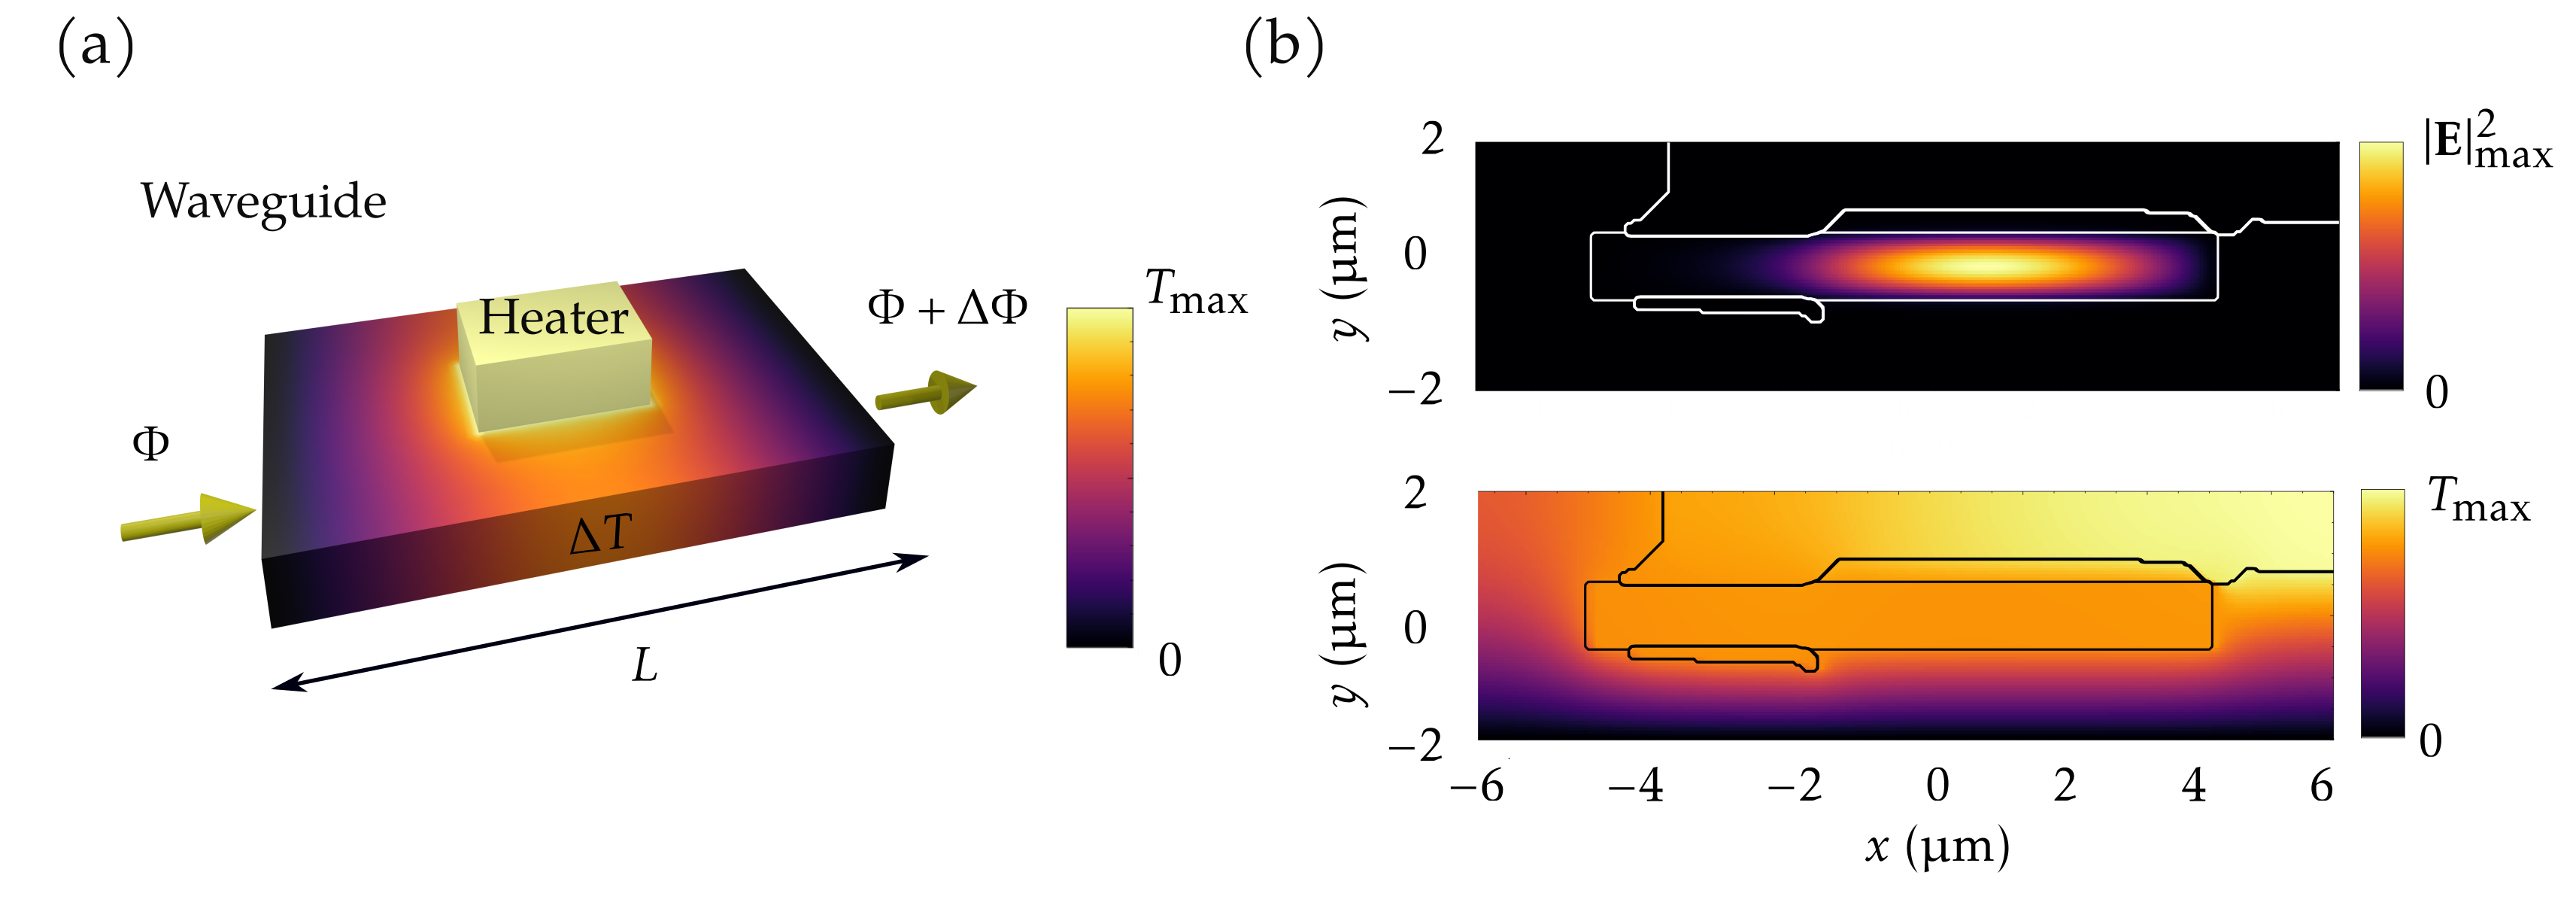
\includegraphics{figures/TOPS_results.png}}%%
    \caption{Topology optimization of thermo-optical phase shifters. (a) Phase-shifting mechanism, where a heater changes the temperature in the waveguide $\Delta T$, inducing a phase shift
    $\Delta \Phi$ over a length $L$. (b) Thermal and optical response of the topology optimized device. Figure adapted with permission from~\cite{ownpub0} © Optical Society of America.}
    \label{fig:thermo_res}
\end{figure}


\subsection*{The effective index via waveguide finite element analysis}

To calculate the phase shift (\eqref{eq:phase_shift}), one needs to find the effective index of an optical mode. This can be done by 
using the finite element formulation for two-dimensional waveguide cross-sections described in~\cite{jin}
\begin{equation}\label{eq:wg_eq}
 \left[\begin{array}{cc}
 A_{\text{tt}}(\varepsilon,k) & 0 \\
    0 & 0
    \end{array}\right]
 \left\{\begin{array}{l}
 E_{\text{t}} \\
 E_z
    \end{array}\right\}
 = -k_z^2
 \left[\begin{array}{cc}
 B_{\text{tt}} & B_{\text{t} z} \\
 B_{z \text{t}} & B_{z z}(\varepsilon,k)
    \end{array}\right]
 \left\{\begin{array}{c}
 E_{\text{t}} \\
 E_z
    \end{array}\right\},
    \end{equation}
where $E_{\text{t}}$ and $E_z$ are the transverse ($x,y$) and longitudinal ($z$) electric field components respectively, $k_z$ is the propagation constant of the optical mode, and $A_{tt}, B_{tt},
B_{zt}$, $B_{tz}$, and $B_{zz}$ are matrices that can be assembled using the shape functions (\eqref{eq:ned_shape})~\cite{jin}. Following~\cite{jin}, we use Nédélec elements (\secref{sec:fem}) for the in-plane components of the electric field and 
Lagrange elements for out-of-plane components. 

Solving the generalized eigenvalue problem in \eqref{eq:wg_eq} yields waveguide modes ($E_t$, $E_z$) and propagation constants ($k_z$). The propagation constant can be rewritten into the \textbf{effective index} $n_\text{eff} = k_z / k$,
 where the real part is a measure of the mode overlap with the refractive index distribution, and the imaginary part ($\Im\{n_\text{eff}\}$) quantifies modal losses. For a numerical implementation of this method, please refer to our GitHub repository~\cite{FEWEC}, which includes a tutorial on solving the 
 generalized eigenvalue problem in \eqref{eq:wg_eq} to find the effective indices and field distributions of waveguide eigenmodes.

 \subsection*{PT-symmetry breaking waveguides}
 Recent progress in waveguide design by Dave and Lipson~\cite{lipson}, proposed the use of \textbf{PT-symmetry breaking} (\secref{sec:nanophotonics}) \textbf{waveguides} as promising candidates for
 thermo-optical phase shifter devices, since they can minimize optical losses while being placed in close contact with (lossy) metallic heaters. To understand this phenomenon, we consider an example with a 
 simulation domain with a $5$ \textmu m height and a $15$ \textmu m width. At the center of a silica cladding ($n\approx 2$) there is a silicon ($n \approx 3.48$) waveguide with a $2$ \textmu m height and 
 a $10$ \textmu m width, where the left half ($x<0$) of the waveguide is lossy [characterized by an extinction coefficient $\kappa>0$ (\eqref{eq:perm})].

\begin{figure}[tb]
    \centering
    \makebox[\textwidth][c]{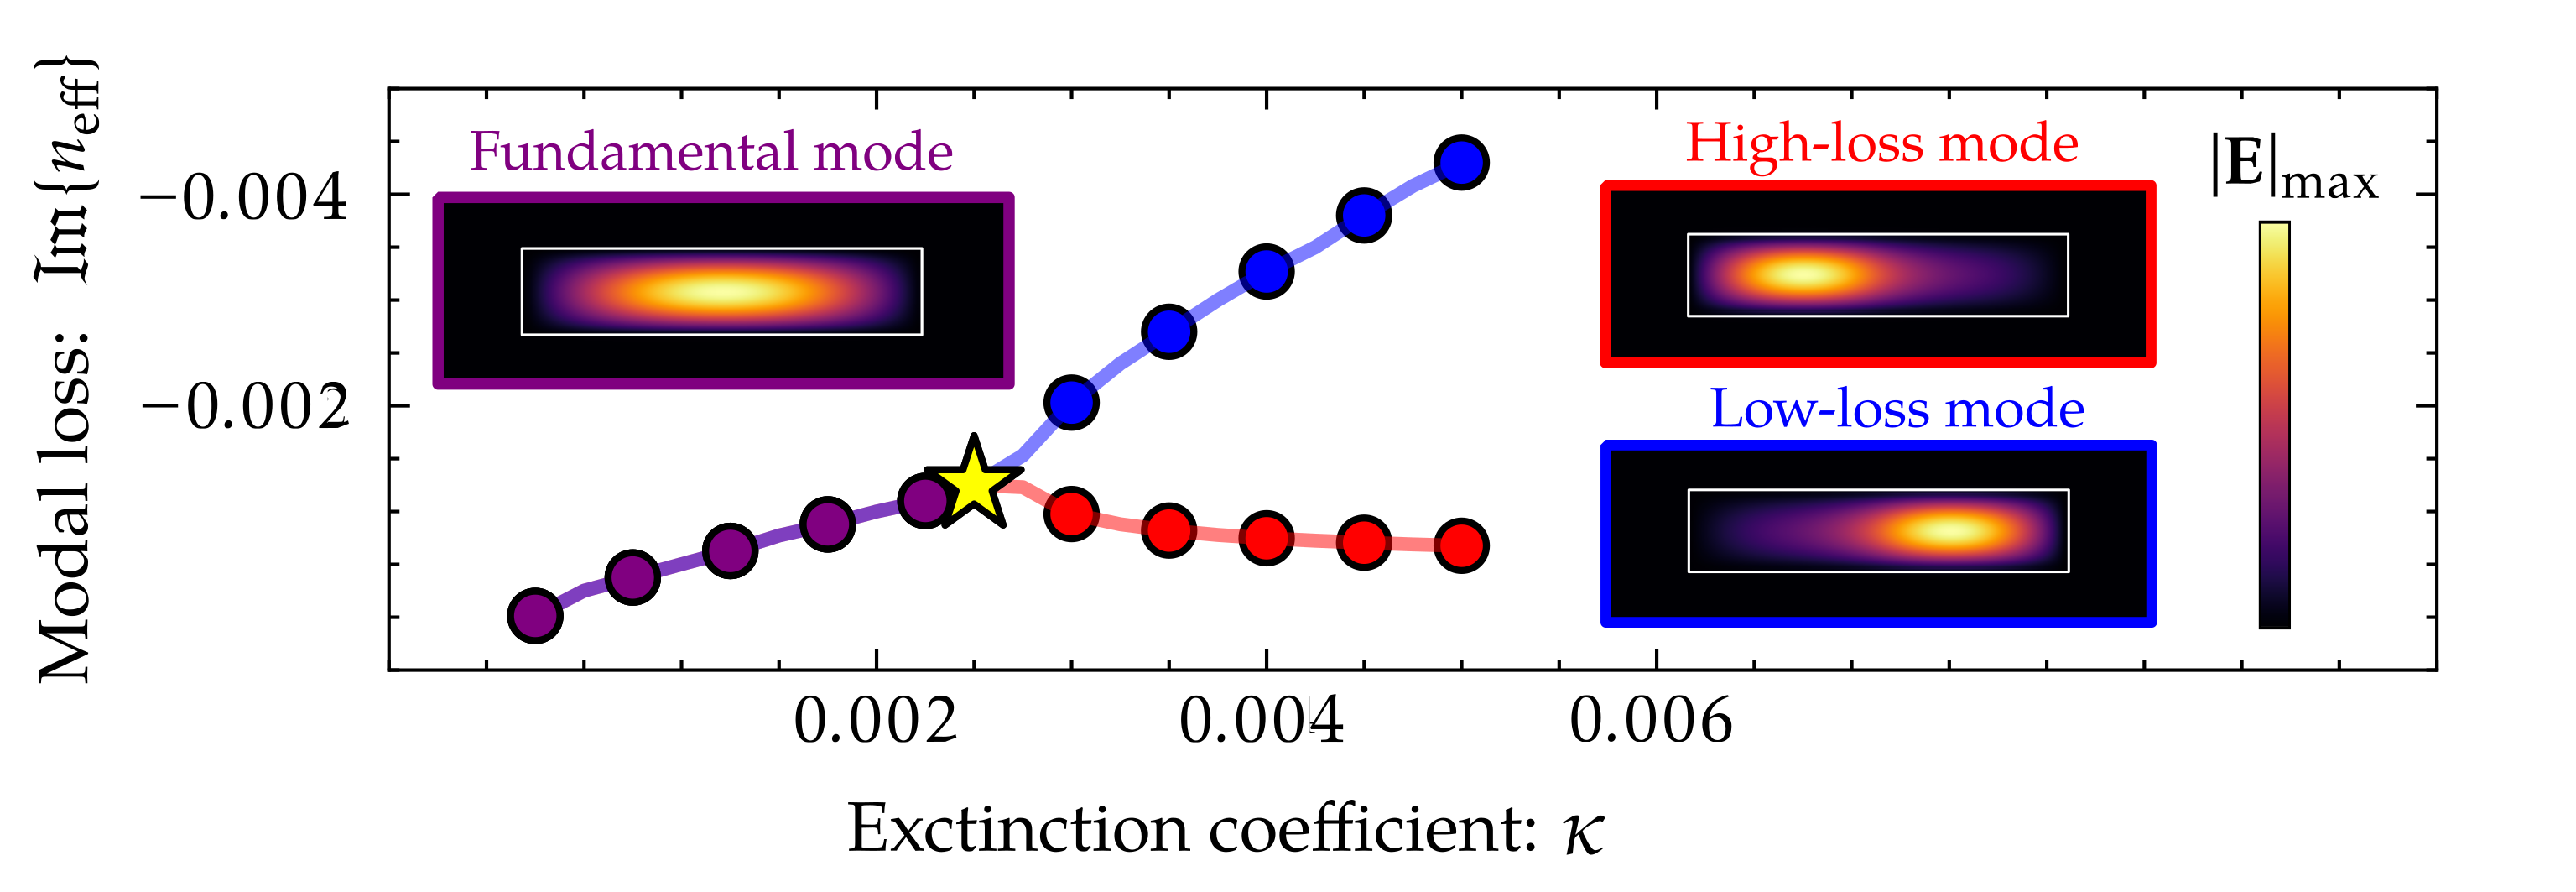
\includegraphics{figures/TOPS_pt.png}}%%
    \caption{Parity-time symmetry breaking mechanism in lossy waveguide modes. The modal losses ($\Im\{n_\text{eff}\}$) as a function of the extinction coefficient ($\kappa$) show the splitting of the fundamental mode into 
    high- and low-loss modes, with their max-normalized electric field norm ($\vert \mathbf{E} \vert$) distribution.}
    \label{fig:pt}
\end{figure}

Using this configuration and perfect electric conductor boundary conditions, we solve the eigenproblem in~\eqref{eq:wg_eq} at the telecom wavelength ($\lambda = 1.55$ \textmu m) for varying extinction coefficients. 
 As shown in~\figref{fig:pt}, increasing the extinction coefficient initially makes the fundamental mode more lossy until a bifurcation (star in~\figref{fig:pt}) splits
  it into high- and low-loss modes. Counter-intuitively, further increasing the extinction coefficient reduces the loss of the low-loss mode 
  because its spatial profile overlaps more strongly with the lossless half of the waveguide.
   This effect is beneficial in thermo-optical waveguide design, since it enables placing a metallic heater in direct contact with the waveguide for better heat transfer while still
    maintaining low optical losses.

\subsection*{Topology optimization results~\cite{ownpub0}}

Inspired by PT-symmetry breaking waveguides, in~\cite{ownpub0}, we use topology optimization to achieve good heat conduction and low optical loss in thermo-optical phase shifters.
The optimization problem considers a waveguide cross-section with a lossy metallic heater, and seeks to find the distribution of metal around the waveguide that minimizes optical loss for both heated and 
unheated configurations. 

Unlike the eigenvalue-based approach presented in the previous section, which estimates losses from the imaginary part of the effective index,
 our method evaluates losses by directly solving a linear system. An optical source excites the waveguide mode, which appears
  as a resonance in the effective index spectrum. The imaginary part of the refractive index ($\Im\{n_\text{eff}\}$) represents the resonance linewidth and therefore the loss:
   the smaller it is, the sharper the resonance and the lower the loss. By maximizing the electric field intensity of the excited mode,
    we can sharpen this resonance and thus minimize losses. Based on this idea, we formulate an optimization problem that designs
     the metallic heater around the waveguide by maximizing the worst-case electric field intensity at two effective indices, representing
      the heated and unheated waveguide states. An example of this is shown in \figref{fig:therm_opt_neff}, where we plot the maximum electric field intensity in the waveguide as a function of 
      the effective index for the optimized device (\figref{fig:thermo_res}) and a reference design in the unheated and heated configurations, showing larger and sharper resonances 
      for the optimized device.
 
      \begin{figure}[b]
         \centering
         \makebox[\textwidth][c]{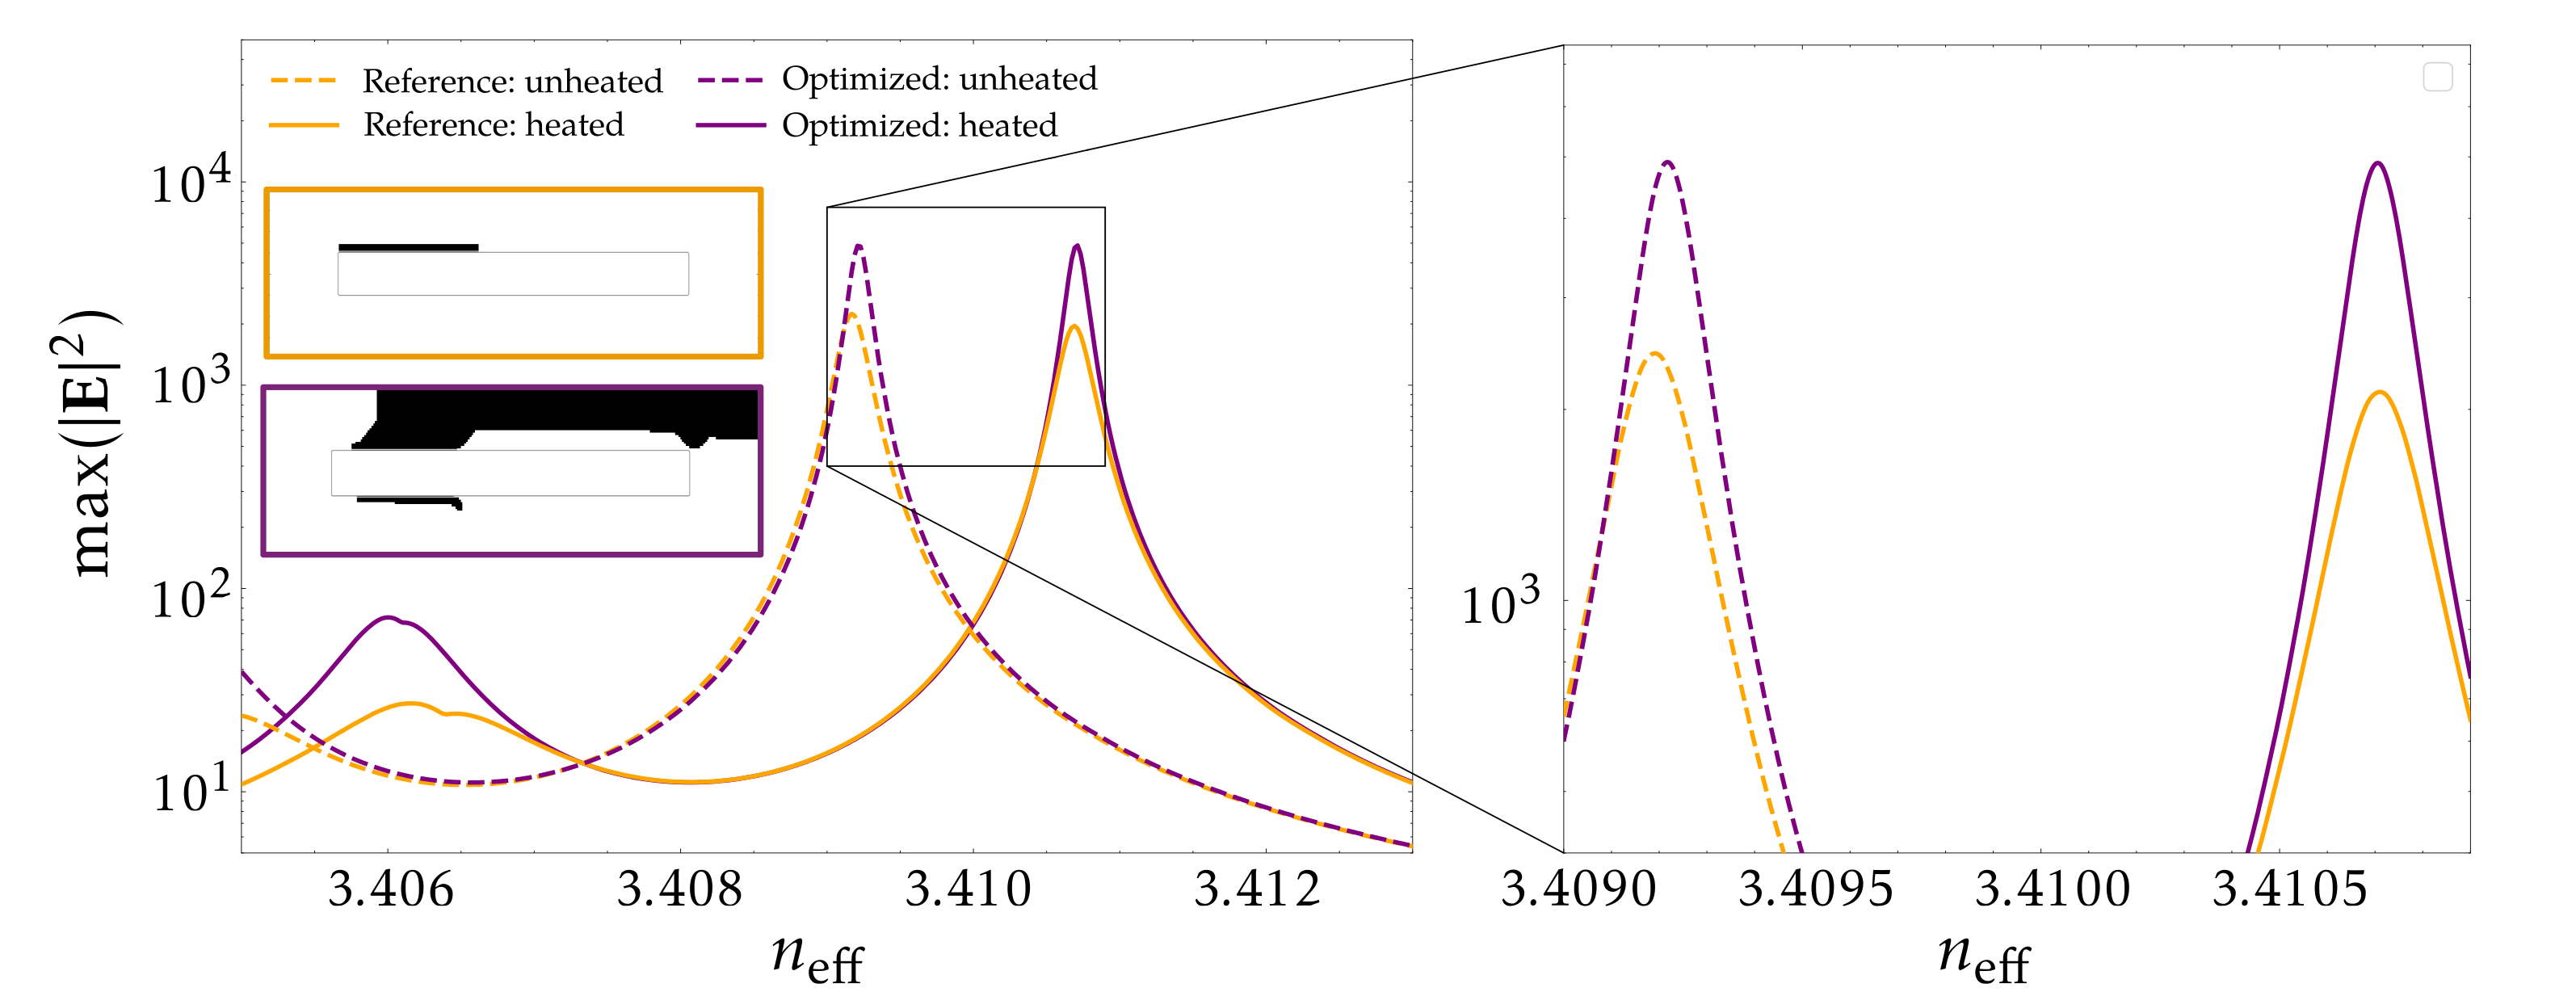
\includegraphics{figures/TOPS_results_2.png}}%%
         \caption{Maximum electric field intensity [$\max(\vert \mathbf{E} \vert^2)$] in the waveguide as a function of the effective index for the topology-optimized and reference designs in the unheated and heated
         configurations. Figure adapted with permission from~\cite{ownpub0} © Optical Society of America.}
         \label{fig:therm_opt_neff}
      \end{figure}
      

 To integrate the heat problem into the 
 topology optimization framework, we use a linear material interpolation 
for the conductivity (Eq. 13 in~\cite{ownpub0}) and an interpolation for the heat source given by $
 Q(\hat{\rho})=P_{\text{in}} \hat{\rho}^p / \left( L A_e \sum^{N_\text{e}}_j \hat{\rho}_j \right)\,,
$
where $P_\text{in}$ is the input power in the heater, $p$ is a penalization factor, $A_e$ is the area of each element, and 
$N_e$ is the total number of elements in the finite element problem. 
This expression models a resistive heater with all material connected in parallel, so that for a fixed input power, the heat 
generation per unit volume increases as the total heater volume decreases.
To solve the inverse design
problem, we derive a coupled adjoint sensitivity analysis~\cite{ownpub0} enabling gradient-based optimization.

Using this framework, we find the results in \figref{fig:therm_opt_neff} and \figref{fig:thermo_res} (b), where we depict the waveguide cross-section with the topology-optimized metallic heater,
allowing the same low-loss mode to propagate in both the heated and unheated scenarios,
reducing optical losses by $\approx 33 \%$ compared to state-of-the-art PT-symmetry breaking thermo-optical phase-shifter proposals (see reference design in \figref{fig:therm_opt_neff})~\cite{lipson}. Similar to the devices
in~\cite{lipson}, the optimized design utilizes the spatially heterogeneous loss profile to engineer an efficient low-loss mode. Using this optimized device as a starting point, several extensions of the topology optimization problem are considered in~\cite{ownpub0}, such as varying volume constraints, optical power, and the inclusion of fabrication constraints (e.g., minimum length scales and layered 
lithography processes).

\subsection*{Outlook and future work}

The framework presented in our work~\cite{ownpub0} provides a foundation for studying and optimizing weakly coupled topology optimization problems. For example, for the design of phase shifters and thermo-optical modulators, it should be straightforward to extend this
formalism to three dimensional system, where one could account for insertion/coupling losses of the integrated photonic circuits. Another example is the use of multi-material topology optimization to design the heating device and the optical waveguide simultaneously. Moreover, this formalism could be applied to design completely different devices, such as re-configurable photonic systems that might be modulated by an external heat source, or thermo-optical
switches based on optical cavities~\cite{switch, switch_2}, where the change in refractive index shifts the cavity in- or out-of-resonance. Lastly, the thermo-optical phase-shifter problem could be
extended to electro-optical phase shifters~\cite{pockels} (\secref{chap:eo}), since the electrostatic Poisson equation $\nabla^2 \phi = -\rho/\varepsilon_0$ is a special case of the heat equation with a spatially homogenous
conduction coefficient, where $\phi$ is the electric potential that replaces the temperature profile. 

\section{Towards strong coupling -- heat dissipation in optics}\label{sec:thermo_strong_coupling}

In the strong coupling regime, the optical response will modify the thermal response, and vice versa.
An example of such an effect is \textbf{optical absorption}, which can lead to significant local heating, altering the refractive index and thus modifying the optical field. 
This mutual dependence requires a strongly coupled treatment of the heat and optical problems (\secref{sec:coupled}), modeled via an electric-field-dependent volumetric heat source~\cite{plasm_heat_source}
\[
Q(\mathbf{r}) = \frac{1}{2} \omega \varepsilon_0 \varepsilon_r^{\prime \prime} |\mathbf{E}(\mathbf{r})|^2,
\]
where the material losses ($\varepsilon_r^{\prime \prime}$) convert the electromagnetic energy into heat. 
This expression is critical for metal nanostructures, where plasmonic resonances cause localized heating~\cite{plasm_heat_source}, and in high-intensity photonics, where even weakly absorbing materials can produce significant heat~\cite{thermal_nl, high_I_T}. Moreover, the thermo-optical feedback can give rise to nonlinear effects (\secref{sec:nanophotonics}), such as self-focusing~\cite{thermal_nl}. If we still consider a linear
thermal response and TOC,
the nonlinearity has the form of a Kerr-type nonlinearity ($\Delta n \propto \vert \mathbf{E} \vert^2$). Accounting for and modeling
these effects could open up the avenue for the inverse design of novel nonlinear thermo-optical devices, with potential applications
in integrated nonlinear photonics~\cite{nl_photonics}, metasurfaces~\cite{nl_meta}, and plasmonics~\cite{novotny}.

\section{Heat transfer as a connectivity constraint}\label{sec:aux}

Lastly, it is worth mentioning that an additional heat equation can be used as an auxiliary equation to enforce connectivity
and structural integrity in topology optimization problems (e.g.,~\cite{vanessa, structural_heat}), which is also exemplified by some of our
works~\cite{ownpub1,ownpub2}. 

This method, introduced in~\cite{li_structural_2016}, is known as the \textbf{virtual temperature method} (VTM). The core idea of the VTM is to simulate a heat transfer problem on an auxiliary thermal field, where the solid domain
 is treated as a heat source and a thermally conductive material. At the same time, void regions are modeled as an
insulating material, and Dirichlet boundary conditions ($T = 0$) are imposed on the boundaries where connectivity is required, while Neuman boundary conditions are imposed
on the rest of boundaries. When 
solving the steady-state heat equation (\eqref{eq:heat}), regions that are disconnected from the boundary 
cannot dissipate heat and therefore attain elevated temperatures. By applying a threshold criterion on the thermal field, such as $T < T_\text{thresh}$, disconnected islands in the design can be 
detected and penalized. For instance, in our works~\cite{ownpub1,ownpub2}, we compute a measure of the total virtual temperature
by integrating the temperature field over the design domain ($\Omega_D$), and add it as a constraint in the optimization problem 
$\int_{\Omega_D} T \d \Omega \leq \epsilon_C$, where $\epsilon_c$ is a sufficiently small constant. Accounting for this constraint in the optimization problem ensures that the final design remains physically connected to the required 
boundaries. 


Note that by appropriately selecting the connecting boundaries it is possible to use the VTM to enforce
(mechanical) structural integrity of the designs~\cite{structural_heat}, which can also be achieved by solving an auxiliary
mechanical problem~\cite{structural_integrity}. For a more robust connectivity constraint formulation with less parameter tuning, we refer the reader to the nonlinear 
virtual temperature method (NVTM)~\cite{nvtm}, and for further details on connectivity constraints, we refer the reader to the review 
article by Cool et al.~\cite{vanessa}.
